We will illustrate the use of RL in medical scenarios with a few motivational examples. These will be recurring examples throughout the report. We summarize these test-cases below.

\subsection{Diabetes}

The first motivating example we state is that of treating diabetes. Diabetes is  a disease that causes a high blood glucose level in patients.
Currently there is no evident cure for this disease \citep{holt2011textbook}. There are two major sub-types of diabetes mellitus: type-1 and type-2. The treatment for diabetes consists of regulating a patient’s
blood glucose level to stay within a specific range. In order to keep their blood glucose level in an acceptable range, type-1 diabetic patients must
inject insulin several times during a day. The amount of insulin that needs to be injected depends on the amount of carbohydrate in the last meal consumed by the patient and current blood glucose level. This is because, when we eat food, our digestive system breaks the carbohydrates down to glucose. The absorption of glucose in the intestine increases its concentration in the blood stream, which puts the body into
a state of hyperglycemia (state of high blood glucose). Glucose, the key source of energy in human body, needs insulin for its routine disposal into cells. In a healthy individual, the pancreas produces
insulin, which allows muscle and fat cells to absorb glucose from blood stream. Consequently the blood glucose level decreases back to the normal level. Other mechanisms operate when the blood glucose goes below its normal value – that is, when the body enters a state of hypoglycemia. The global situation of diabetes afflicting people is shown in Figure \ref{Fig:Diabetes-IDF}.


\begin{figure}[!th]
\center
\begin{tabular}{cc}
\subfigure[2.75\textwidth][Diabetes Scenario Worldwide] 
    %with $r_{i_{{i}\neq {*}}}=0.07$ and $r^{*}=0.1$
    {
\includegraphics[scale=0.3]{img/diabetes_idf.png}
%\caption{Diabetes Scenario Worldwide}
\label{Fig:Diabetes-IDF}
}
&
\subfigure[2.75\textwidth][Sepsis severity resulting in death] 
    %with $r_{i_{{i}\neq {*}}}=0.07$ and $r^{*}=0.1$
    {
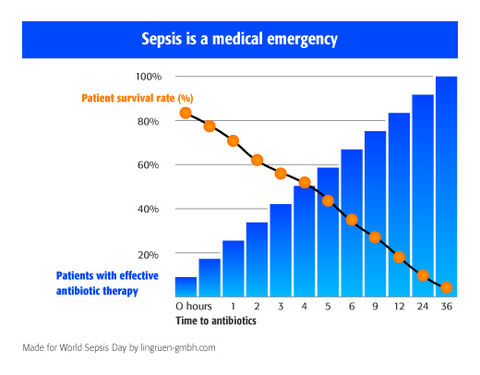
\includegraphics[scale=0.3]{img/sepsis-antibiotics.jpg}
%\caption{Sepsis severity resulting in death}
\label{Fig:Sepsis-Antibiotics}
}
\end{tabular}
\caption{Severity of Diabetes and Sepsis}
\end{figure}

\subsection{Sepsis}

Our second motivating example is sepsis treatment in ICU. Sepsis is a complication of an infection resulting out of an extreme immune system response triggering widespread inflammation throughout the body. Sepsis can range from mild to severe and because it can be potentially life-threatening, it requires sustained and immediate medical attention. Sepsis treatment varies and depends on the cause of the infection that led to sepsis, as well as the severity of symptoms. Because mild sepsis can rapidly progress to severe sepsis and then septic shock, doctors must work quickly to reduce inflammation. Common treatments for sepsis include: 1. administering Antibiotics 2. injecting Intravenous (IV) Fluids and 3. in the extreme cases when blood pressure has fallen dangerously low using Vasopressors. An illustrative figure showing the severity of sepsis leading to death resulting from delay in administering antibiotics is shown in Figure \ref{Fig:Sepsis-Antibiotics}.

%\begin{figure}[!th]
%\center
%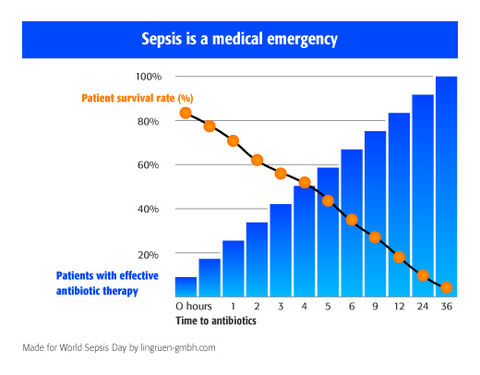
\includegraphics[scale=0.4]{img/sepsis-antibiotics.jpg}
%\caption{Sepsis severity resulting in death}
%\label{Fig:Sepsis-Antibiotics}
%\end{figure}